\documentclass[a4paper,12pt]{scrartcl}

\usepackage[utf8]{inputenc}
\usepackage[T1]{fontenc}
\usepackage{url}
\usepackage{graphicx}

\newcounter{zad}
\newcounter{pkt}

\newcommand{\zad}{\vspace{4mm}\noindent\setcounter{pkt}{0}\stepcounter{zad}{\bf \thezad.} }
\newcommand{\zadgw}{\vspace{4mm}\noindent\setcounter{pkt}{0}\stepcounter{zad}{\bf \thezad$^*$.} }
\newcommand{\pkt}{\vspace{1mm}\stepcounter{pkt}\alph{pkt}) }

\begin{document}

\section*{Projekt - zaliczenie dotychczas przerobionego materiału}

Jeżeli nie masz jeszcze konta na stronie \url{main.edu.pl}, to je załóż.

\subsection*{Rozgrzewka: Gra w trzy pytania}

Zaimplementuj program, który odgaduje dowolną liczbę od 0 do 7, zadając trzy pytania
 zgodnie z poniższym diagramem.

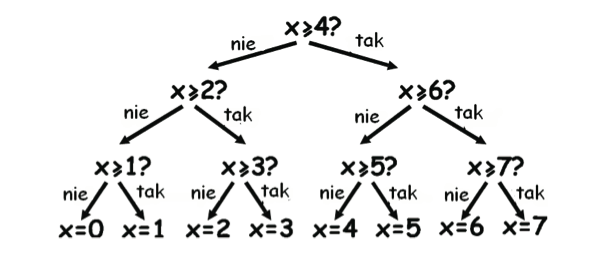
\includegraphics[width=\textwidth]{drzewo_3pytania.png}

Gotowe rozwiązanie wyślij na adres \url{andrzej.nagorko@sternik.edu.pl}.

\subsection*{Dwa zadania na zajęcia}

\begin{enumerate}
\item \url{http://main.edu.pl/pl/user.phtml?op=showtask&task=prz&con=PAS}
\item \url{http://main.edu.pl/pl/user.phtml?op=showtask&task=min&con=PAS}
\end{enumerate}

Gotowe rozwiązania wyślij na adres \url{andrzej.nagorko@sternik.edu.pl}.

\newpage
\section*{Zadanie domowe: punkty do liceum}

Twoim zadaniem jest napisanie programu, który oblicza liczbę punktów kwalifikacyjnych do liceum, w zgodzie z poniższą specyfikacją.

\subsection*{Twoje zadanie}

\begin{enumerate}
\item Przeczytaj poniższy tekst {\sc do końca} ze zrozumieniem.
\item {\sc Na kartce} zaplanuj pytania, które zadasz kandydatowi oraz ich kolejność. 
  Zwróć uwagę, że nie zawsze będziesz zadawał te same pytania!
\item Napisz program.
\item {\sc Przetestuj} program.
\item Wyślij kod programu na adres \url{andrzej.nagorko@sternik.edu.pl}
\item Za {\sc dobrze} napisany program wysłany {\sc przed końcem zajęć} oferuję ocenę celującą z informatyki.
\item Możecie pracować w parach. Powodzenia!
\end{enumerate}

\section*{Specyfikacja}
\subsection*{Zasady punktacji przy kwalifikowaniu kandydatów}

Opracowane na podstawie zasad kwalifikacji do IX LO w Szczecinie.

\subsubsection*{Zasady ogólne}

\begin{tabular}{|l|l|}
\hline egzamin gimnazjalny & max. 100 punktów \\
\hline wyniki uzyskane na świadectwie ukończenia gimnazjum & max. 60 punktów \\
\hline kryteria dodatkowe & max. 40 punktów \\
\hline
\end{tabular}

\vspace{3mm}
Laureaci konkursów przedmiotowych o zasięgu wojewódzkim i ponadwojewódzkim, których program obejmuje w całości lub poszerza treści podstawy programowej z co najmniej jednego przedmiotu, 
przyjmowani są do szkoły, niezależnie od ustalonych kryteriów*.

Kandydat może uzyskać razem maksymalnie 200 punktów.

W przypadku klas dwujęzycznych: klasy z językiem francuskim oraz klasy z językiem niemieckim jako drugim językiem nauczania, kandydat dodatkowo uzyskuje punkty ze sprawdzianu uzdolnień kierunkowych, lub z egzaminu gimnazjalnego z języka na poziomie rozszerzonym - maksymalnie 50 punktów.

Kandydat do klasy dwujęzycznej może uzyskać razem maksymalnie 250 punktów.

\subsubsection*{Zasady szczegółowe}

Punkty za wyniki egzaminu gimnazjalnego przeprowadzanego w ostatnim roku gimnazjum-0,2 pkt za każdy punkt procentowy uzyskany na egzaminie gimnazjalnym z zakresów: 

\begin{itemize}
  \item języka polskiego (20 pkt),
  \item historii i wiedzy o społeczeństwie (20 pkt),
  \item matematyki (20 pkt),
  \item przedmiotów przyrodniczych (20 pkt),
  \item języka obcego nowożytnego na poziomie podstawowym (20 pkt).
\end{itemize}

Kandydat może uzyskać razem maksymalnie 100 punktów.

\vspace{5mm}
Świadectwo szkolne - oceny z czterech przedmiotów:

\vspace{5mm}
{
\footnotesize
\begin{tabular}{|l|l|l|}
\hline
\rule{0pt}{2em}Profil klasy &
\rule{0pt}{2em}\begin{minipage}{5cm}
Przedmioty nauczane w zakresie rozszerzonym 
\end{minipage} &
\rule{0pt}{2em}
\begin{minipage}{5cm}
Przedmioty, których oceny są uwzględniane w rekrutacji 
\end{minipage}
\\
\hline
Informatyczna (A)
&
\begin{minipage}{5cm}
matematyka,\\
język obcy nowożytny,\\
informatyka
\end{minipage}
&
\rule{0pt}{3em}\begin{minipage}{5cm}
język polski\\
matematyka\\
język obcy nowożytny \\
informatyka
\end{minipage}
\\
\hline
\begin{minipage}{3,2cm}
Dwujęzyczna (B)
\end{minipage}
&
\begin{minipage}{5cm}
Matematyka,\\
język francuski, \\
wiedza o społeczeństwie,\\
geografia
\end{minipage}
&
\rule{0pt}{3em}
\begin{minipage}{5cm}
język polski,\\
matematyka,\\
język obcy nowożytny,\\
geografia
\end{minipage}
\\
\hline
Humanistyczna (C)
&
\begin{minipage}{5cm}
język polski,\\
historia,\\
język obcy nowożytny
\end{minipage}
&
\rule{0pt}{3em}
\begin{minipage}{5cm}
język polski,\\
matematyka,\\
język obcy nowożytny,\\
historia
\end{minipage}
\\
\hline
\end{tabular}
}

\vspace{5mm}
Wszystkie oceny z w/w przedmiotów przeliczane są na punkty zgodnie z zasadą:

\begin{itemize}
\item celujący - 15 punktów;
\item bardzo dobry - 12 punktów;
\item dobry - 9 punktów;
\item dostateczny - 5 punktów;
\end{itemize}

Kandydat może uzyskać razem maksymalnie 60 punktów.

\subsection*{Kryteria dodatkowe}

\begin{itemize}
\item Laureaci jednego i więcej konkursów organizowanych przez Towarzystwo na Rzecz Młodzieży Uzdolnionej (20 punktów)

\item Finaliści jednego i więcej konkursów przedmiotowych organizowanych przez Kuratorium Oświaty  oraz Towarzystwo na Rzecz Młodzieży Uzdolnionej oraz Olimpiad  dla Gimnazjalistów przeprowadzanych  na zlecenie Ministerstwa Edukacji Narodowej (15 punktów)

\item Laureaci Konkursu Wiedzy o Kulturze Świata Antycznego (20 punktów)

\item Finaliści Konkursu Wiedzy o Kulturze Świata Antycznego (15 punktów)

\item Ukończenie gimnazjum z wyróżnieniem (5 punktów)

\item Kandydat może uzyskać razem maksymalnie:  35 punktów za osiągnięcia w konkursach i 5 punktów za ukończenie gimnazjum z wyróżnieniem.
\end{itemize}

\subsection*{*Wykaz konkursów}

\footnotesize
Konkursy organizowane przez Kuratorium Oświaty:

\begin{itemize}
\item Konkurs Polonistyczny;
\item Konkurs Matematyczny;
\item Konkurs Fizyczny z elementami astronomii;
\item Konkurs Chemiczny;
\item Konkurs Biologiczny;
\item Konkurs Historyczny z elementami wiedzy o społeczeństwie;
\item Konkurs Geograficzny;
\item Konkurs Języka Angielskiego;
\item Konkurs Języka Niemieckiego;
\end{itemize}
Olimpiady przeprowadzane na zlecenie Ministerstwa Edukacji Narodowej:
\begin{itemize}
\item {\bf Olimpiada Matematyczna dla Gimnazjalistów;}
\item {\bf Olimpiada Informatyczna dla Gimnazjalistów;}
\item Olimpiada Języka Angielskiego dla Gimnazjalistów;
\end{itemize}

\end{document}
